%%% Hlavní soubor. Zde se definují základní parametry a odkazuje se na ostatní části. %%%

%% Verze pro jednostranný tisk:
% Okraje: levý 40mm, pravý 25mm, horní a dolní 25mm
% (ale pozor, LaTeX si sám přidává 1in)
\documentclass[12pt,a4paper]{report}
\setlength\textwidth{145mm}
\setlength\textheight{247mm}
\setlength\oddsidemargin{15mm}
\setlength\evensidemargin{15mm}
\setlength\topmargin{0mm}
\setlength\headsep{0mm}
\setlength\headheight{0mm}
% \openright zařídí, aby následující text začínal na pravé straně knihy
\let\openright=\clearpage

%% Pokud tiskneme oboustranně:
% \documentclass[12pt,a4paper,twoside,openright]{report}
% \setlength\textwidth{145mm}
% \setlength\textheight{247mm}
% \setlength\oddsidemargin{14.2mm}
% \setlength\evensidemargin{0mm}
% \setlength\topmargin{0mm}
% \setlength\headsep{0mm}
% \setlength\headheight{0mm}
% \let\openright=\cleardoublepage

%% Vytváříme PDF/A-2u
\usepackage[a-2u]{pdfx}

%% Přepneme na českou sazbu a fonty Latin Modern
\usepackage[czech]{babel}
\usepackage{lmodern}
\usepackage[T1]{fontenc}
\usepackage{textcomp}

%% Použité kódování znaků: obvykle latin2, cp1250 nebo utf8:
\usepackage[utf8]{inputenc}

%%% Další užitečné balíčky (jsou součástí běžných distribucí LaTeXu)
\usepackage{amsmath}        % rozšíření pro sazbu matematiky
\usepackage{amsfonts}       % matematické fonty
\usepackage{amsthm}         % sazba vět, definic apod.
\usepackage{bbding}         % balíček s nejrůznějšími symboly
			    % (čtverečky, hvězdičky, tužtičky, nůžtičky, ...)
\usepackage{bm}             % tučné symboly (příkaz \bm)
\usepackage{graphicx}       % vkládání obrázků
\usepackage{fancyvrb}       % vylepšené prostředí pro strojové písmo
\usepackage{indentfirst}    % zavede odsazení 1. odstavce kapitoly
\usepackage{natbib}         % zajištuje možnost odkazovat na literaturu
			    % stylem AUTOR (ROK), resp. AUTOR [ČÍSLO]
\usepackage[nottoc]{tocbibind} % zajistí přidání seznamu literatury,
                            % obrázků a tabulek do obsahu
\usepackage{icomma}         % inteligetní čárka v matematickém módu
\usepackage{dcolumn}        % lepší zarovnání sloupců v tabulkách
\usepackage{booktabs}       % lepší vodorovné linky v tabulkách
\usepackage{paralist}       % lepší enumerate a itemize
\usepackage{xcolor}         % barevná sazba

% dodané mimo šablonu
\usepackage{graphicx}		% umisti obrazky vedle sebe
\usepackage{subcaption}		% umisti obrazky vedle sebe
\usepackage{enumitem}
\usepackage{dirtree}		% pro strom adresářů příloh
\usepackage{hyperref}
%\usepackage[cache=false]{minted}			% syntax highlight
%\usepackage{algpseudocode}  
%\usepackage{algorithm}
\usepackage{multicol}

\usepackage[shortcuts]{extdash}		% pro možnost zakázání dělení slov kolem pomlčky
									% např. pro slovo "chce-li", které lze zapsat "che\=/li"

%%% Údaje o práci

% Název práce v jazyce práce (přesně podle zadání)
\def\NazevPrace{Analyzátor USB paketů}

% Název práce v angličtině
\def\NazevPraceEN{USB Packet Analyzer}

% Jméno autora
\def\AutorPrace{Peter Lakatoš}

% Rok odevzdání
\def\RokOdevzdani{2021}

% Název katedry nebo ústavu, kde byla práce oficiálně zadána
% (dle Organizační struktury MFF UK, případně plný název pracoviště mimo MFF)
\def\Katedra{Katedra distribuovaných a~spolehlivých systémů}
\def\KatedraEN{Department of~Distributed and~Dependable Systems}

% Jedná se o katedru (department) nebo o ústav (institute)?
\def\TypPracoviste{Katedra}
\def\TypPracovisteEN{Department}

% Vedoucí práce: Jméno a příjmení s~tituly
\def\Vedouci{Mgr.~Pavel Ježek,~Ph.D.}

% Pracoviště vedoucího (opět dle Organizační struktury MFF)
\def\KatedraVedouciho{Katedra distribuovaných a~spolehlivých systémů}
\def\KatedraVedoucihoEN{Department of~Distributed and~Dependable Systems}

% Studijní program a obor
\def\StudijniProgram{Informatika}
\def\StudijniObor{Programování a~softwarové systémy}

% Nepovinné poděkování (vedoucímu práce, konzultantovi, tomu, kdo
% zapůjčil software, literaturu apod.)
\def\Podekovani{%
Poděkování.
}

% Abstrakt (doporučený rozsah cca 80-200 slov; nejedná se o zadání práce)
\def\Abstrakt{%
USB zbernica je dnes jedným z najrozšírenejších spôsobov pripojenia periférií k počítaču. 
Cieľom práce bolo vytvoriť software, ktorý analyzuje zachytenú komunikáciu medzi zariadnením pripojeným na danú zbernicu a počítačom.

Aplikácia následne rozumným spôsobom vizuálne zobrazuje zanalyzované dáta. Počiatočná verzia sa špecificky zameriava na HID triedu zariadení a ponúka aj sémantický význam jej úzkej podmnožiny do ktorej patria myš, klávesnica a joystick. Pri vizuálnej reprezentácii dát sa práca sa inšpiruje rôznymi dostupnými softwarmi, pričom rozlične kombinuje resp. dopĺňa ich vlastnosti a implementuje z nich tie, ktoré vníma ako najlepšie riešenie v danej situácii.

Ďalšie vlastnosti aplikácie sú napríklad parsovanie HID Report Descriptoru vďaka ktorému je jednoduchšie pridať sémantickú analýzu rôznym ďalším HID zariadeniam. Celkový návrh aplikácie by mal ponúknuť možnosť budúcej implementácie ďalších USB tried pre prípadné rozšírenie.
}
\def\AbstraktEN{%
Abstract.
}

% 3 až 5 klíčových slov (doporučeno), každé uzavřeno ve složených závorkách
\def\KlicovaSlova{%
{USB} {HID}
}
\def\KlicovaSlovaEN{%
{key} {words}
}

%% Balíček hyperref, kterým jdou vyrábět klikací odkazy v PDF,
%% ale hlavně ho používáme k uložení metadat do PDF (včetně obsahu).
%% Většinu nastavítek přednastaví balíček pdfx.
\hypersetup{unicode}
\hypersetup{breaklinks=true}

%% Definice různých užitečných maker (viz popis uvnitř souboru)
%%% Tento soubor obsahuje definice různých užitečných maker a prostředí %%%
%%% Další makra připisujte sem, ať nepřekáží v ostatních souborech.     %%%

%%% Drobné úpravy stylu

% Tato makra přesvědčují mírně ošklivým trikem LaTeX, aby hlavičky kapitol
% sázel příčetněji a nevynechával nad nimi spoustu místa. Směle ignorujte.
\makeatletter
\def\@makechapterhead#1{
  {\parindent \z@ \raggedright \normalfont
   \Huge\bfseries \thechapter. #1
   \par\nobreak
   \vskip 20\p@
}}
\def\@makeschapterhead#1{
  {\parindent \z@ \raggedright \normalfont
   \Huge\bfseries #1
   \par\nobreak
   \vskip 20\p@
}}
\makeatother

% Toto makro definuje kapitolu, která není očíslovaná, ale je uvedena v obsahu.
\def\chapwithtoc#1{
\chapter*{#1}
\addcontentsline{toc}{chapter}{#1}
}

% Trochu volnější nastavení dělení slov, než je default.
\lefthyphenmin=2
\righthyphenmin=2

% Zapne černé "slimáky" na koncích řádků, které přetekly, abychom si
% jich lépe všimli.
\overfullrule=1mm

%%% Makra pro definice, věty, tvrzení, příklady, ... (vyžaduje baliček amsthm)

\theoremstyle{plain}
\newtheorem{veta}{Věta}
\newtheorem{lemma}[veta]{Lemma}
\newtheorem{tvrz}[veta]{Tvrzení}

\theoremstyle{plain}
\newtheorem{definice}{Definice}

\theoremstyle{remark}
\newtheorem*{dusl}{Důsledek}
\newtheorem*{pozn}{Poznámka}
\newtheorem*{prikl}{Příklad}

%%% Prostředí pro důkazy

\newenvironment{dukaz}{
  \par\medskip\noindent
  \textit{Důkaz}.
}{
\newline
\rightline{$\qedsymbol$}
}

%%% Prostředí pro sazbu kódu, případně vstupu/výstupu počítačových
%%% programů. (Vyžaduje balíček fancyvrb -- fancy verbatim.)

\DefineVerbatimEnvironment{code}{Verbatim}{fontsize=\small, frame=single}

%%% Prostor reálných, resp. přirozených čísel
\newcommand{\R}{\mathbb{R}}
\newcommand{\N}{\mathbb{N}}

%%% Užitečné operátory pro statistiku a pravděpodobnost
\DeclareMathOperator{\pr}{\textsf{P}}
\DeclareMathOperator{\E}{\textsf{E}\,}
\DeclareMathOperator{\var}{\textrm{var}}
\DeclareMathOperator{\sd}{\textrm{sd}}

%%% Příkaz pro transpozici vektoru/matice
\newcommand{\T}[1]{#1^\top}

%%% Vychytávky pro matematiku
\newcommand{\goto}{\rightarrow}
\newcommand{\gotop}{\stackrel{P}{\longrightarrow}}
\newcommand{\maon}[1]{o(n^{#1})}
\newcommand{\abs}[1]{\left|{#1}\right|}
\newcommand{\dint}{\int_0^\tau\!\!\int_0^\tau}
\newcommand{\isqr}[1]{\frac{1}{\sqrt{#1}}}

%%% Vychytávky pro tabulky
\newcommand{\pulrad}[1]{\raisebox{1.5ex}[0pt]{#1}}
\newcommand{\mc}[1]{\multicolumn{1}{c}{#1}}


%% Titulní strana a různé povinné informační strany
\begin{document}
%%% Titulní strana práce a další povinné informační strany

%%% Titulní strana práce

\pagestyle{empty}
\hypersetup{pageanchor=false}

\begin{center}

\centerline{\mbox{
\includegraphics[width=166mm]{img/logo-cs.pdf}}}

\vspace{-8mm}
\vfill

{\bf\Large BAKALÁŘSKÁ PRÁCE}

\vfill

{\LARGE\AutorPrace}

\vspace{15mm} 

{\LARGE\bfseries\NazevPrace}

\vfill

\Katedra

\vfill

{
\centerline{\vbox{\halign{\hbox to 0.45\hsize{\hfil #}&\hskip 0.5em\parbox[t]{0.45\hsize}{\raggedright #}\cr
Vedoucí bakalářské práce:&\Vedouci \cr
\noalign{\vspace{2mm}}
Studijní program:&\StudijniProgram \cr
\noalign{\vspace{2mm}}
Studijní obor:&\StudijniObor \cr
}}}}

\vfill

% Zde doplňte rok
Praha \RokOdevzdani

\end{center}

\newpage

%%% Následuje vevázaný list -- kopie podepsaného "Zadání bakalářské práce".
%%% Toto zadání NENÍ součástí elektronické verze práce, nescanovat.

%%% Strana s čestným prohlášením k bakalářské práci

\openright
\hypersetup{pageanchor=true}
\pagestyle{plain}
\pagenumbering{roman}
\vglue 0pt plus 1fill

\noindent
Prohlašuji, že jsem tuto bakalářskou práci vypracoval(a) samostatně a výhradně
s~použitím citovaných pramenů, literatury a dalších odborných zdrojů.
Tato práce nebyla využita k získání jiného nebo stejného titulu.

\medskip\noindent
Beru na~vědomí, že se na moji práci vztahují práva a povinnosti vyplývající
ze zákona č. 121/2000 Sb., autorského zákona v~platném znění, zejména skutečnost,
že Univerzita Karlova má právo na~uzavření licenční smlouvy o~užití této
práce jako školního díla podle §60 odst. 1 autorského zákona.

\vspace{10mm}

\hbox{\hbox to 0.5\hsize{%
V \hbox to 6em{\dotfill} dne \hbox to 6em{\dotfill}
\hss}\hbox to 0.5\hsize{\dotfill\quad}}
\smallskip
\hbox{\hbox to 0.5\hsize{}\hbox to 0.5\hsize{\hfil Podpis autora\hfil}}

\vspace{20mm}
\newpage

%%% Poděkování

\openright

\noindent
\Podekovani

\newpage

%%% Povinná informační strana bakalářské práce

\openright

\vbox to 0.5\vsize{
\setlength\parindent{0mm}
\setlength\parskip{5mm}

Název práce:
\NazevPrace

Autor:
\AutorPrace

\TypPracoviste:
\Katedra

Vedoucí bakalářské práce:
\Vedouci, \KatedraVedouciho

Abstrakt:
\Abstrakt

Klíčová slova:
\KlicovaSlova

\vss}
\newpage \openright %\nobreak
\vbox to 0.49\vsize{
\setlength\parindent{0mm}
\setlength\parskip{5mm}

Title:
\NazevPraceEN

Author:
\AutorPrace

\TypPracovisteEN:
\KatedraEN

Supervisor:
\Vedouci, \KatedraVedoucihoEN

Abstract:
\AbstraktEN

Keywords:
\KlicovaSlovaEN

\vss}

\newpage

\openright
\pagestyle{plain}
\pagenumbering{arabic}
\setcounter{page}{1}


%%% Strana s automaticky generovaným obsahem bakalářské práce

\tableofcontents

%%% Jednotlivé kapitoly práce jsou pro přehlednost uloženy v samostatných souborech
\chapter{Úvod}

USB je najrozšírenejšia zbernica na pripojenie rôznych periférií k počítaču. Vznikla v druhej polovici 90. rokov 20. storočia, kedy boli rôzne zariadenia a ich porty veľmi úzko mapované. Na pripojenie základných zariadení ako myš alebo klávesnica slúžil napríklad sériový port PS/2~\cite{ps2_port}. K pripojeniu tlačiarne sa často používal paralelný port Centronics~\cite{parallel_port}. Ešte pred PS/2 portom sa myš pripájala cez veľmi známy sériový port RS-232~\cite{rs232_port}. Všetky tieto porty boli typu \textit{point-to-point} -- na jeden port je možné pripojiť len jedno zariadenie. Toto sa paralelným portom dalo čiastočné obísť tým, že niektoré zariadenia podporovali tzv. \textit{daisy chain} -- do pripojeného zariadenia sa pripojí ďalšie zariadenie, do toho sa pripojí ďalšie, atď. (napríklad typická tlačiareň toto nepodporovala, takže musela byť pripojená na konci \textit{daisy chainu}). Existovala takisto paralelná \textit{SCSI} zbernica~\cite{scsi_hub}, ktorej návrh bol prispôsobený aby podporoval  \textit{daisy chain}. Tá fungovala dobre na zariadeniach ako externé HDD a skenery, ale bola nepraktická pre zariadenia ako myš a klávesnica.

USB vzniklo za účelom nahradiť a zjednotiť tieto spôsoby pripojenia bežných periférií k počítaču. Návrh zbernice je založený na hviezdicovej topológii, ktorá umožňuje cez jeden port pripojiť až 127 zariadení súčasne. Z toho vyplýva, že USB interface v sebe zahŕňa obrovskú množinu protokolov, ktoré sú hierarchicky usporiadané. K analýze paketov ktoré sa pohybujú na danej zbernici nám slúžia tzv. USB paket analyzátory. Tie môžu mať podobu hardwarového zariadenia, alebo softwarovej aplikácie. Môžu slúžiť napríklad ako učebná pomôcka pre účel lepšieho pochopenia jednotlivých protokolov. Takisto sa často využívajú pri implementácii vlastného USB zariadenia na ladenie komunikácie medzi daným zariadením a driverom. Využitie ale majú aj v opačnom prípade, keď implementujeme vlastný driver a potrebujeme sledovať jeho komunikáciu s konkrétnym zariadením. Cieľom tejto práce bude naprogramovať funkčný softwarový USB analyzátor, ktorý by mal presnejšie slúžiť práve ako učebná pomôcka pre lepšie pochopenie určitej množiny protokolov. Cieľová platforma aplikácie bude Windows.

\section{Základné pojmy}

V tejto sekcii si vysvetlíme niektoré základné pojmy ktoré budeme neskôr v~texte používať.

\begin{figure}[!htb]
	\centering
	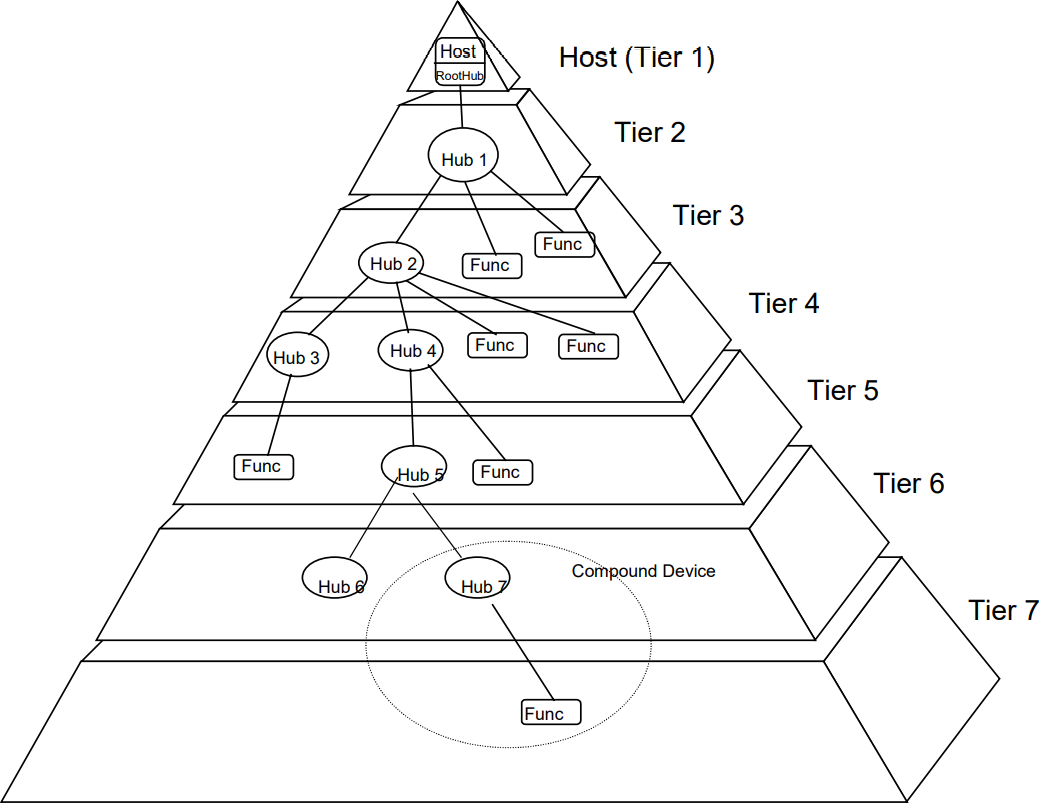
\includegraphics[width=\textwidth]{img/uvod_usb_topology}
	\caption{USB topológia. Obrázok prevzatý z USB 2.0 špecifikácie~\cite{usb_topology}.}
	\label{obr:uvod:usb_topology}
\end{figure}

Ako sme už vyššie spomínali a ako ilustruje obrázok~\ref{obr:uvod:usb_topology}, USB zbernica je založená na vrstevnatej hviezdicovej topológii. Na vrchu všetkého sa nachádza \textbf{USB Host}~\cite{usb_host} čo je systém do ktorého sa pripájajú ostatné USB zariadenia (v našom prípade je \textit{USB Host} počítač). \textbf{USB zariadenie}~\cite{usb_device} je buď:
\begin{itemize}
\item \textbf{Hub}~\cite{usb_hub} -- poskytuje dodatočné pripojenia k USB zbernici.
\item \textbf{Funkcia}~\cite{usb_function} -- poskytuje novú funkcionalitu systému (napríklad joystick, reproduktory, myš a pod.)
\end{itemize}

 V každom USB systéme sa nachádza práve jeden \textit{USB Host}. Ten má integrovaný tzv. \textbf{Root Hub}~\cite{usb_host}, ktorý poskytuje možné body pripojenia pre ďalšie zariadenia. Interface medzi hostom a USB sa nazýva \textbf{Host Controller}~\cite{usb_host}. Vzhľadom na niektoré časové obmedzenia USB je maximálny počet vrstiev 7 (vrátane \textit{USB Host} vrstvy). Každý káblový segment je \textit{point-to-point}~\cite{usb_bus_topology} spojenie medzi:
\begin{itemize}
\item \textit{host} $\longleftrightarrow$ \textit{hub}/\textit{funkcia}
\item \textit{hub} $\longleftrightarrow$ \textit{hub}/\textit{funkcia}
\end{itemize}

USB zariadenia využívajú tzv. \textbf{descriptory} na predávanie informácií o sebe samých. \textbf{Descriptor}~\cite{usb_descriptor} je dátová štruktúra s predom definovaným formátom. Existuje viacero typov \textit{USB descriptorov} (device, endpoint, interface atď.), ktorých význam si vysvetlíme neskôr.

Vzhľadom na hierarchickú štruktúru USB protokolov sa \textit{USB zariadenia} delia na rôzne triedy~\cite{usb_classes}. USB trieda je zoskupenie zariadení (alebo interfacov) ktoré majú spoločné vlastnosti alebo funkcionalitu. Tieto triedy umožňujú USB hostovi identifikovať dané zariadenie a jeho funkcionalitu. Každá trieda má svoju vlastnú \textit{Class Specification} -- definuje správanie zariadení v jednotlivých triedach a opisuje ich komunikačný protokol, ktorý sa naprieč triedami líši. Takisto definuje rôzne descriptory, ktoré sú špecifické pre danú triedu. Príklady USB tried a jednotlivých zariadení ktoré do nich patria sú:
\begin{itemize}
\item Mass Storage (napr. SD karta a flash disk)
\item Audio (napr. reproduktory a slúchadlá)
\item HID -- Human Interface Device (napr. myš, klávesnica alebo joystick)
\end{itemize}

\textbf{Paket}~\cite{usb_packet} je súbor dát zoskupený na prenos po zbernici. Typicky sa skladá z troch častí:
\begin{itemize}
\item základné informácie o danom pakete (napríklad zdroj, cieľ, dĺžka) -- takisto nazývané hlavička paketu
\item samotné dáta
\item detekcia chýb, opravné bity
\end{itemize}

Komunikácia na zbernici medzi \textit{USB hostom} a \textit{zariadením} prebieha práve pomocou prenosu \textit{USB paketov}.   Existujú 4 typy takýchto prenosov~\cite{usb_type_transfers}:
\begin{itemize}
\item \textbf{Control Transfer} -- používa sa na nakonfigurovanie USB zariadenia v momente keď sa pripojí na zbernicu.
\item \textbf{Bulk Data Transfer} -- typicky pozostáva z väčšieho množstva dát ktoré sú posielané nárazovo (využívajú ho najmä tlačiarne alebo skener). Vďaka detekcii chýb na hardwarovej úrovni je zaistená správnosť prenesených dát.
\item \textbf{Interrupt Data Transfer} -- spoľahlivý prenos ktorý sa využíva hlavne na odovzdávanie aktuálnych informácií (ako napríklad pohyb myšou). Tieto informácie musia byť doručené USB zbernicou za čas kratší ako má špecifikované dané zariadenie.
\item \textbf{Isochronous Data Transfer} -- takisto nazývaný ako streaming v reálnom čase. Typický príklad je prenos zvuku.
\end{itemize}

Našu aplikáciu by sme chceli zamerať na Windows a tak si vysvetlíme ešte zopár špecifických pojmov, ktoré sa viažu na túto kokrétnu platformu.

Podľa MSDN dokumentácie~\cite{usbclientdriver} je \textbf{USB client driver} software nainštalovaný na počítači, ktorý komunikuje s USB zariadením aby spojazdnil jeho funkcionalitu. Žiaden \textit{USB client driver} ale nemôže priamo komunikovať so svojím zariadením. Namiesto toho vytvorí požiadavku, súčasťou ktorej je dátová štruktúra nazývaná \textbf{URB}~\cite{usburb} (USB Request Block). Tá opisuje detaily požiadavku, takisto ako aj status o jeho vykonaní.

Na záver si ešte zadefinujeme rozdiel medzi \textit{USB paket analyzátorom} a \textit{USB paket snifferom}. Pod pojmom \textbf{USB paket sniffer} budeme rozumieť aplikáciu, ktorá monitoruje dianie na USB zbernici a je schopná ho rozumným spôsobom ukladať v predom definovanom formáte. Ako \textbf{USB paket analyzátor} budeme brať aplikáciu ktorá je schopná rozanalyzovať USB pakety (istým spôsobom ich vyobraziť alebo ukázať ich sémantický význam) uložené v predom definovanom formáte. Bežne sa tieto pojmy označujú za jednu a tú istú vec, aj keď ich funkcionalita spolu nijako priamočiaro nesúvisí a existujú nástroje, ktoré vedia len jedno alebo druhé. Preto dáva zmysel ich od seba explicitne oddeliť.

Momentálne by sme mali chápať všetky základné pojmy týkajúce sa USB, a tak si poďme trochu bližšie objasniť zameranie našej aplikácie. Našu aplikáciu zameriavame výukovým smerom pre programátorov, ktorí chcú lepšie pochopiť komunikáciu na USB zbernici. Z toho dôvodu by sme v nej určite chceli zahrnúť analýzu základných USB descriptorov, ktoré sú bližšie definované v špecifikácii USB 2.0~\cite{usbdoc} v~kapitole 9.6. Keďže chceme bližšie priblížiť komunikáciu na danej zbernici, potrebujeme konkrétne zariadenia, s ktorými ju budeme analyzovať. Dáva dobrý zmysel si zvoliť zariadenia, ktoré každý z nás dobre pozná, má ich k dispozícii a bežne ich využíva. Zároveň by ale mali mať dostatočne jednoduchý komunikačný protokol. Práve preto sa s našou aplikáciou zameriame na užšiu podmnožinu HID zariadení, konkrétne myš, klávesnica a joystick. Vzhľadom na zameranie našej aplikácie výukovým smerom prikladáme najväčšiu prioritu samotnej analýze dát.  Z dôvodu celkovej univerzality USB je z didaktického hľadiska ťažké nasimulovať jednotný príklad u každého študenta zvlášť. Už len obyčajná myš, aj keď je to jedno zariadenie, má od rôznych výrobcov inak nadefinované správanie a posiela dáta v rozličných formátoch. Preto je pre nás dôležité vedieť analyzovať pakety, ktoré si učiteľ predpripraví, skontroluje ich didaktickú správnosť a uloží do súboru. Podpora živého zachytávania paketov a ich analýzy je tak v našom programe najmenej dôležitá.

Keďže sa v našej práci budeme venovať hlavne analýze HID zariadení, tak si túto USB triedu rozoberieme trochu detailnejšie.

\subsection*{HID}
\label{uvod:sec:HID}

Podľa dodatku k USB špecifikácii~\cite{usbhid} je \textbf{HID} (z anglického \uv{Human Interface Device}) USB trieda pozostávajúca prevažne zo zariadení, ktoré sú využívané človekom na riadenie určitých systémovových aplikácií. Medzi najpoužívanejšie príklady patrí myš, klávesnica alebo joystick.

Ako sme už spomínali vyššie, jednotlivé USB triedy majú definované vlastné descriptory špecifické pre danú triedu. Jedným z takýchto descriptorov je aj \textit{Report Descripor}. Ten popisuje dáta, ktoré generuje konkrétne zariadenie. Analýzou \textit{Report Descriporu} sme schopní určiť veľkosť a kompozíciu dát posielaných zariadením. Z toho vyplýva, že komunikácia HID zariadením s USB hostom sa môže líšiť nie len vo veľkosti posielaných dát, ale takisto aj v ich význame.

Lepšie to uvidíme na konkrétnom príklade. K dispozícii máme 2 rozdielne myši -- Genius DX\=/120~\cite{genius_mouse} a Logitech G502 Proteus Spectrum~\cite{logitech_mouse}

\begin{figure}[!htb]
\centering
\begin{subfigure}{.5\textwidth}
  \centering
  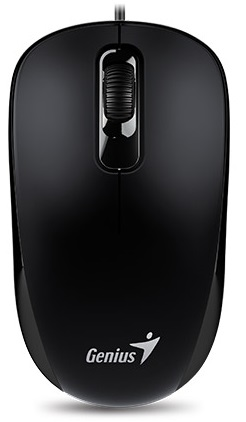
\includegraphics[width=.4\linewidth]{img/genius_mys.jpg}
  \caption{Fotka genius myši prevzatá z oficiálnej genius stránky~\cite{genius_mouse_pic}}
  \label{obr:uvod:genius:mouse:pic}
\end{subfigure}%
\begin{subfigure}{.5\textwidth}
  \centering
  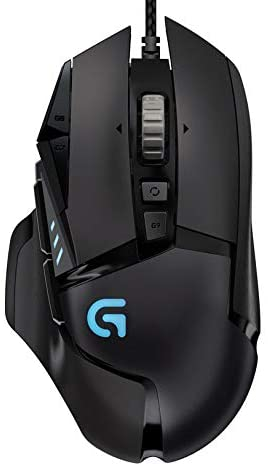
\includegraphics[width=.4\linewidth]{img/logitech_mys}
  \caption{Fotka logitech myši prevzatá zo stránky obchodu~\cite{logitech_mouse_pic}}
  \label{fig:sub2}
\end{subfigure}
\caption{Ukážka myší, ktorých input budeme porovnávať}
\label{obr:uvod:logitech:mouse:pic}
\end{figure}

Teraz si ukážeme ako sa líši ich input. Dáta budeme vyobrazovať pomocou obyčajného hexdumpu (zvýraznená časť v hexdumpe reprezentuje input zariadenia). Na oboch myšiach stlačíme ľavé tlačidlo a mierne ich posunieme smerom hore. Dáta, ktoré poslala genius myš sú vyobrazené na obrázku~\ref{obr:uvod:genius:input} a dáta poslané logitech myšou môžeme vidieť na obrázku~\ref{obr:uvod:logitech:input}.

\begin{figure}[!htb]
	\centering
	
\includegraphics[width=12cm]{img/uvod_genius_input}
	\caption{Ukážka hexdumpu so zvýrazneným inputom genius myši.}
	\label{obr:uvod:genius:input}
\end{figure}

\begin{figure}[!htb]
	\centering
	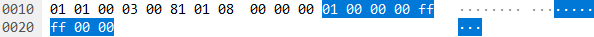
\includegraphics[width=12cm]{img/uvod_logitech_input}
	\caption{Ukážka hexdumpu so zvýrazneným inputom logitech myši.}
	\label{obr:uvod:logitech:input}
\end{figure}

Aj napriek tomu, že sa jedná o zariadenia z tej istej USB triedy a dokonca o rovnaké zariadenie -- myš,  má ich komunikácia rozličný tvar definovaný priamo výrobcom zariadenia. Analýzou \textit{Report Descriporu} (o ktorej si viac povieme neskôr v práci) sme zistili, že dáta, ktoré poslala genius myš majú nasledujúci význam:
\begin{itemize}
\item Byte 0: bity 0--2 reprezentujú stlačenie jednotlivých tlačidiel, bity 3--7 tvoria len dodatočnú výplň bytu
\item Byte 1: reprezentuje súradnicu X
\item Byte 2: reprezentuje súradnicu Y
\item Byte 3: reprezentuje koliesko myši
\end{itemize}

Pre porovnanie, význam dát poslaných logitech myšou je nasledovný:
\begin{itemize}
\item Byte 0--1: reprezentujú stlačenie jednotlivých tlačidiel
\item Byte 2--3: reprezentuje súradnicu X
\item Byte 4--5: reprezentuje súradnicu Y
\item Byte 6: reprezentuje koliesko myši
\item Byte 7: je rezervovaný výrobcom myši
\end{itemize}

Vizuálne zobrazený význam dát genius myši je ukázaný na obrázku~\ref{obr:uvod:genius:input:vyznam} a logitech myši na obrázku~\ref{obr:uvod:logitech:input:vyznam}.

\begin{figure}[!htb]
	\centering
	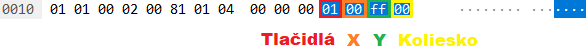
\includegraphics[width=12cm]{img/uvod_genius_input_vyznam}
	\caption{Ukážka hexdumpu so zvýrazneným inputom genius myši s významom.}
	\label{obr:uvod:genius:input:vyznam}
\end{figure}

\begin{figure}[!htb]
	\centering
	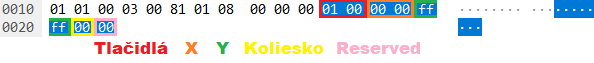
\includegraphics[width=12cm]{img/uvod_logitech_input_vyznam}
	\caption{Ukážka hexdumpu so zvýrazneným inputom logitech myši s významom.}
	\label{obr:uvod:logitech:input:vyznam}
\end{figure}

Z toho vyplýva, že aby sme boli schopní vykonať sémantickú analýzu HID zariadení, bude pre nás kľúčové vedieť rozparsovať \textit{Report Descripor} a na základe toho interpretovať input zariadení.

\section{Existujúce aplikácie}

Momentálne existuje niekoľko známych aplikácií ktoré slúžia na analýzu USB paketov. Ich predbežným skúmaním a používaním sme ale zistili, že úplne nevyhovujú našim konkrétnym požiadavkám. Avšak mnohé ich funkcie nám prídu užitočné a môžu poslúžiť ako inšpirácia v implementovaní našej aplikácie. V tejto kapitole si ukážeme výhody a nevýhody zopár aplikácií, ktoré sme si zvolili ako príklady v oblasti paket analyzátorov. Ich výber spočíval v tom, že sú veľmi rozšírené medzi verejnosťou a sú najbližšie k tomu čo by sme chceli od našej aplikácie.

Je nutné upozorniť, že väčšina dnešných analyzátorov sú platené aplikácie, prípadne majú odomknuté len základné vlastnosti s~možnosťou dokúpenia si plnej verzie. Práve preto sme nemali možnosť si pri všetkých vyskúšať ich celú funkcionalitu a na niektoré platené funkcie máme tak len ilustračný pohľad.


\subsection*{Wireshark}
\label{uvod:sec:Wireshark}

Aplikácia, ktorá na prvý pohľad nesúvisí s USB zbernicou. Wireshark je pravdepodobne najznámejší analyzátor a sniffer sieťových paketov. Jeho funkcionalita je veľmi rozsiahla, a~vzhľadom na~to, že sa jedná o~open-source projekt, neustále rastie. Vďaka jeho obecnému návrhu podporuje spoluprácu s~rôznymi inými sniffermi (LANalyzer, NetXRay a pod.). Jeden z~takýchto snifferov je \textit{USBPcap}, ktorý zachytáva USB komunikáciu a tým pádom je Wireshark schopný analyzovať pakety aj nad~touto zbernicou. 

Pre priblíženie niektorých funkcií Wiresharku si ukážeme analýzu komunikácie s USB myšou (Genius DX\=/120~\cite{genius_mouse}). Medzi tie úplne základné funkcie určite patrí hexdump dát nad~ktorými prebieha analýza, ktorý je vyobrazený na obrázku~\ref{obr:uvod:wireshark_hexdump}. 

\begin{figure}[!htb]
	\centering
	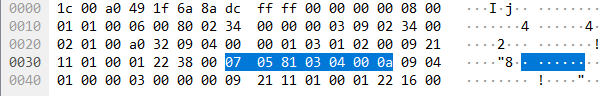
\includegraphics[width=12cm]{img/uvod_wireshark_hexdump}
	\caption{Ukážka hexdumpu vo Wiresharku.}
	\label{obr:uvod:wireshark_hexdump}
\end{figure}


Tento hexdump je tvorený dátami z jedného control prenosu, kde zariadenie posiela informácie o sebe samom v podobe rôznych descriptorov. 

V hexdumpe si takisto vieme pomocou kliknutia a ťahania myšou označiť ľubovoľné dáta, ktoré chceme. Zvýraznené byty na obrázku~\ref{obr:uvod:wireshark_hexdump_endpoint} reprezentujú jeden \textit{endpoint descriptor}.

\begin{figure}[!htb]
	\centering
	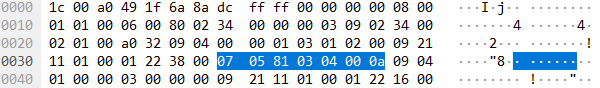
\includegraphics[width=12cm]{img/uvod_wireshark_hexdump_endpoint}
	\caption{Ukážka hexdumpu so zvýrazneným endpoint descriptorom.}
	\label{obr:uvod:wireshark_hexdump_endpoint}
\end{figure}

Pri pohybe myšou nad daným hexdumpom ponúka Wireshark interaktívnu odozvu, pričom farebne oddeľuje jednotlivé byty podľa ich významu. Na obrázku~\ref{obr:uvod:wireshark_hexdump_data_selection} vidíme konkrétny príklad -- ak podržíme myš nad hexa časťou bytu 00, automaticky nám to označí aj byte 04 pred ním, pretože spoločne reprezentujú jednotnú informáciu -- položku \textit{wMaxPacketSize} v \textit{endpoint descriptore}.

\begin{figure}[!htb]
	\centering
	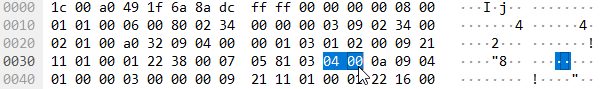
\includegraphics[width=12cm]{img/uvod_wireshark_data_selection}
	\caption{Ukážka hexdumpu s farebným oddelením na základe významu.}
	\label{obr:uvod:wireshark_hexdump_data_selection}
\end{figure}

Ďalšia užitočná vlastnosť je, že pri označení hexa znakov v hexdumpe, sa samé označia aj im odpovedajúce tlačiteľné znaky (obdobne to funguje aj opačným smerom). To, že vyššie označených 7 bytov na obrázku~\ref{obr:uvod:wireshark_hexdump_endpoint} reprezentujú \textit{endpoint descriptor} sme zistili vďaka špecifikácii jednotlivých descriptorov a vlastnou analýzou bytov v hexdumpe. Wireshark ale ponúka rozličné zobrazenie tých istých dát, a to napríklad aj pomocou stromovej štruktúry, ktorá už jednotlivým bytom pridáva ich sémantický význam v slovnom tvare ako je ukázané na obrázku~\ref{obr:uvod:tree_structure} nižšie.

\begin{figure}[!htb]
	\centering
	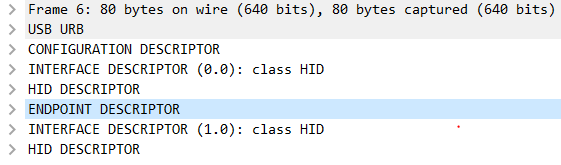
\includegraphics[width=11cm]{img/uvod_tree_structure}
	\caption{Ukážka reprezentácie dát pomocou stromovej štruktúry.}
	\label{obr:uvod:tree_structure}
\end{figure}

 Jednotlivé položky si môžeme bližšie rozbaliť. Napríklad vyššie zvýraznených 7 bytov reprezentujú konkrétny \textit{endpoint descriptor}, ktorý je ukázaný na obrázku~\ref{obr:uvod:endpoint}. Na tom istom obrázku si takisto môžeme všimnúť, že položka \textit{wMaxPacketSize} má hodnotu 4, čo je presne hodnota bytov 04 00, ktoré sme spomínali vyššie na obrázku~\ref{obr:uvod:wireshark_hexdump_data_selection}

\begin{figure}[!htb]
	\centering
	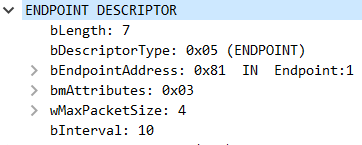
\includegraphics[width=8cm]{img/uvod_endpoint}
	\caption{Endpoint descriptor reprezentovaný dátami zvýraznenými na obrázku~\ref{obr:uvod:wireshark_hexdump} vyššie.}
	\label{obr:uvod:endpoint}
\end{figure}

Medzi viac špecifické funkcie patrí detailnejšie vyobrazenie jednotlivých bytov a~ich význam, ako je možné vidieť nižšie na~obrázku~\ref{obr:uvod:byte_detail_foto}. Na tomto obrázku vidíme rozbalenú položku \textit{bEndpointAddress}, ktorej hodnota je 0x81. Siedmy bit tejto hodnoty reprezentuje smer endpointu (IN -- slúži na prenos dát device $\longrightarrow$ host, OUT opačne) a dolné 4 bity označujú číslo endpointu. Túto vlastnosť aj napriek jej využitiu mnohé konkurenčné aplikácie postrádajú.

\begin{figure}[!htb]
	\centering
	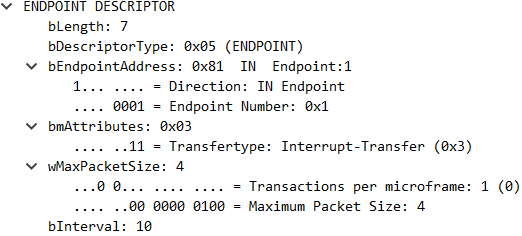
\includegraphics[width=8cm]{img/uvod_byte_detail}
	\caption{Ukážka vyobrazenia jednotlivých bytov.}
	\label{obr:uvod:byte_detail_foto}
\end{figure}

Wireshark ponúka interaktívne užívateľské rozhranie. V prípade kliknutia na konkrétny byte v hexdumpe sa nám označí jemu odpovedajúca položka v stromovej štruktúre. Príklad je ukázaný na obrázku~\ref{obr:uvod:hexdump_click}.

\begin{figure}[!htb]
	\centering
	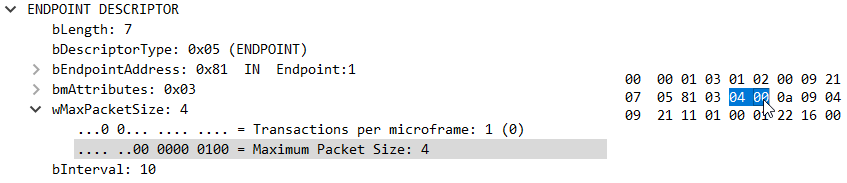
\includegraphics[width=\textwidth]{img/uvod_wireshark_hexdump_click}
	\caption{Ukážka kliknutia na položku v hexdumpe.}
	\label{obr:uvod:hexdump_click}
\end{figure}

Podobne to funguje aj opačne, takže ak klikneme na položku v stromovej štruktúre, označí sa jej odpovedajúca časť v hexdumpe. Príklad kliknutia na \textit{endpoint descriptor} v stromovej štruktúre a označenia jemu odpovedajúcej časti hexumpu je vidieť na obrázku~\ref{obr:uvod:tree_click}.

\begin{figure}[!htb]
	\centering
	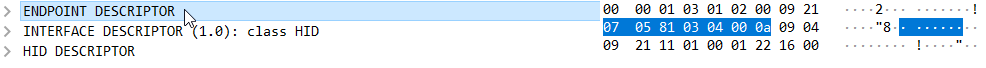
\includegraphics[width=\textwidth]{img/uvod_wireshark_tree_click}
	\caption{Ukážka kliknutia na položku \textit{endpoint descriptoru} v stromovej štruktúre.}
	\label{obr:uvod:tree_click}
\end{figure}

Obecné vyobrazenie pohybu paketov na zbernici bez hlbšej analýzy je ukázané na obrázku~\ref{obr:uvod:wireshark_listview} nižšie.

\begin{figure}[!htb]
	\centering
	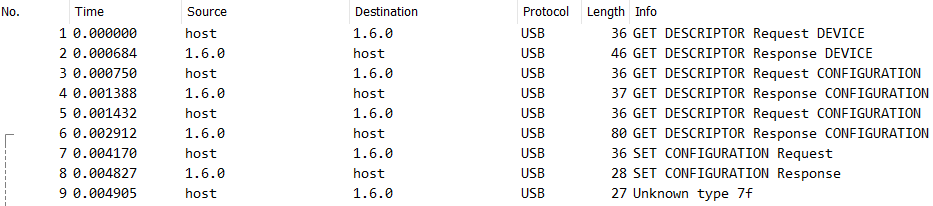
\includegraphics[width=\textwidth]{img/uvod_wireshark_listview}
	\caption{Príklad obecného vyobrazenia jednotlivých paketov vo Wiresharku.}
	\label{obr:uvod:wireshark_listview}
\end{figure}

Výhoda Wiresharku je hlavne v~tom, že podporuje širokú škálu descriptorov a~plná verzia programu je dostupná úplne zadarmo. Z~pohľadu užívateľa je až prekvapivé, že aj~napriek rozsiahlosti programu je aplikácia veľmi user-friendly orientovaná a~dopĺňa ju intuitívne užívateľské rozhranie.

Naopak, jeho nevýhodou je sčasti neprehľadný hexdump. Ako môžeme vidieť na obrázku~\ref{obr:uvod:wireshark_hexdump}, jedná sa o obyčajný hexdump, ktorý nijakým spôsobom neoddeľuje význam dát bez interakcie užívateľa. Preto v momente ak by sme nemali stromovú štruktúru k odpovedajúcemu hexdumpu, museli by sme sa riadiť špecifikáciou a vlastnou analýzou. V prípade rozsiahlejšieho hexdumpu môže byť veľmi obtiažné sa v ňom potom zorientovať. Ďalšia vec ktorá nám nevyhovuje, je chýbajúca sémantická analýza inputu rôznych zariadení. Ten je vyobrazený len pomocou hexdumpu a popisu \uv{Leftover Capture Data} ako je ukázané na obrázku~\ref{obr:uvod:wireshark_input}. Zo sekcie~\ref{uvod:sec:HID} nám je teda jasné, že vôbec netušíme čo jednotlivé dáta znamenajú, pretože ich význam je definovaný v \textit{Report Descriptore}.

\begin{figure}[!htb]
	\centering
	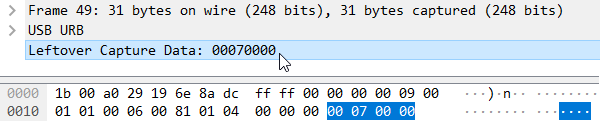
\includegraphics[width=12cm]{img/uvod_wireshark_input}
	\caption{Príklad inputu myši vo Wiresharku.}
	\label{obr:uvod:wireshark_input}
\end{figure}

\subsection*{Device Monitoring Studio}

Aplikácia ponúka analýzu sieťových a~USB paketov, tak ako aj~analýzu komunikácie prebiehajúcej cez~sériový port. Zároveň slúži aj ako sniffer na všetkých týchto portoch.

Ako prvé na~aplikácii zaujme spôsob zvolenia si zariadenia s~ktorým bude sledovaná komunikácia. Je implementovaný štýlom stromovej štruktúry ako je ukázané na~obrázku~\ref{obr:uvod:hhd_treeview_foto}~nižšie, kde máme konkrétne označenú rovnakú myš s ktorou komunikáciu sme sledovali predchádzajúcim programom. 

\begin{figure}[!htb]
	\centering
	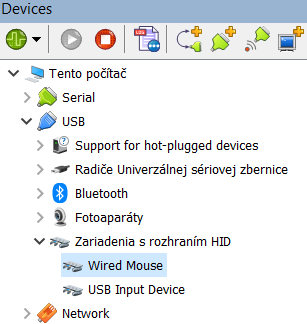
\includegraphics{img/uvod_hhd_treeview}
	\caption{Ukážka stromovej štruktúry na~zvolenie si zariadenia, s~ktorým bude zachytávaná komunikácia.}
	\label{obr:uvod:hhd_treeview_foto}
\end{figure}

Základná verzia programu ponúka vizuálne zobrazenie \textit{URB}, tak ako aj analýzu jednotlivých paketov.
Pod analýzou si tu môžeme predstaviť ale len obyčajný hexdump, ktorý neposkytuje žiadne významové oddelenie dát a tým pádom je obtiažnejšie sa v ňom zorientovať. Príklad môžeme vidieť na obrázku~\ref{obr:uvod:hhd_hexdump}.

\begin{figure}[!htb]
	\centering
	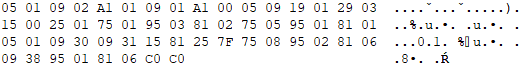
\includegraphics[width=12cm]{img/uvod_hhd_hexdump}
	\caption{Príklad hexdumpu v Device Monitoring Studio.}
	\label{obr:uvod:hhd_hexdump}
\end{figure}


Takisto tu nemáme kompletné sémantické vysvetlenie čo dané dáta znamenajú (napríklad pomocou stromovej štruktúry ako to rieši konkurencia). K dispozícii máme len veľmi obmedzený popis jednotlivých paketov (číslo paketu, device request, a pod.), pričom ani nie je veľmi jasné odkiaľ sa tieto informácie vzali. Príklad takéhoto popisu aj s hexdumpom je ukázaný na obrázku~\ref{obr:uvod:hhd_analyza}~nižšie.

\begin{figure}[!htb]
	\centering
	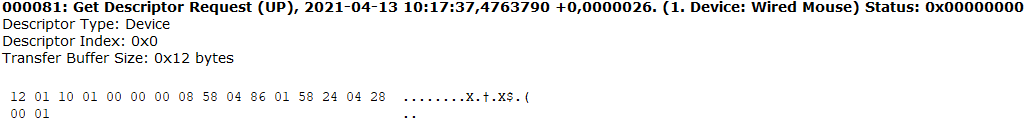
\includegraphics[width=\textwidth]{img/uvod_hhd_analyza}
	\caption{Príklad analýzy paketov.}
	\label{obr:uvod:hhd_analyza}
\end{figure}


Vyobrazenie \textit{URB} (obrázok~\ref{obr:uvod:hhd_urb}~) tak ponúka súhrn týchto popisov jednotlivých paketov, ktoré sú postupne zachytené počas komunikácie na zbernici.

\begin{figure}[!htb]
	\centering
	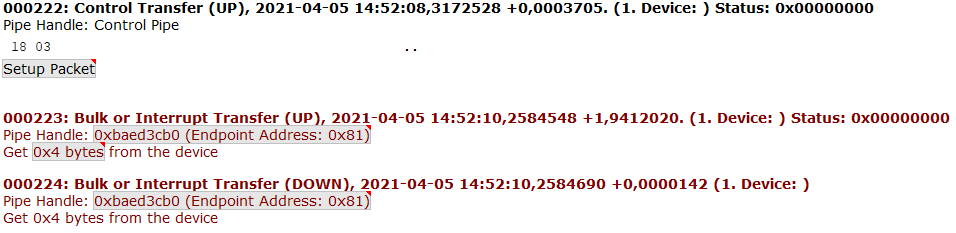
\includegraphics[width=\textwidth]{img/uvod_hhd_urb}
	\caption{Ukážka vyobrazenia URB.}
	\label{obr:uvod:hhd_urb}
\end{figure}

Pričom pri dvojkliku na šedé časti textu (napríklad \textit{Setup Packet} alebo \textit{Endpoint Address}) sa užívateľovi rozbalí okno s detailnejším popisom.
 
Analýza inputu myši, ktorú môžeme vidieť na obrázku~\ref{obr:uvod:hhd_input}, je riešená podobným spôsobom ako pri analýze descriptorov.

\begin{figure}[!htb]
	\centering
	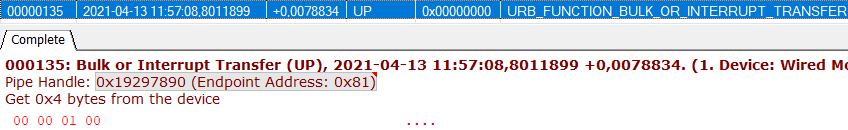
\includegraphics[width=\textwidth]{img/uvod_hhd_input}
	\caption{Príklad inputu myši v Device Monitoring Studio.}
	\label{obr:uvod:hhd_input}
\end{figure}

Obecné vyobrazenie jednotlivých paketov bez bližšej analýzy je riešené podobne ako vo Wiresharku, pričom pakety sú farebne oddelené podľa ich smeru pohybu na zbernici (posielané smerom host $\longrightarrow$ zariadenie/smerom zariadenie $\longrightarrow$ host). Toto je veľmi pekná funkcionalita, ktorá celkovo sprehľadňuje komunikáciu zariadenia s hostom. Príklad je ukázaný na obrázku~\ref{obr:uvod:hhd_listview}.

\begin{figure}[!htb]
	\centering
	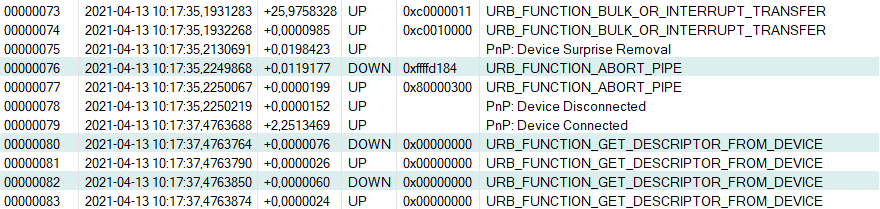
\includegraphics[width=\textwidth]{img/uvod_hhd_listview}
	\caption{Príklad obecného vyobrazenia jednotlivých paketov v Device Monitoring Studio.}
	\label{obr:uvod:hhd_listview}
\end{figure}

Zaujímavá funkcionalita, ktorú ale program ponúka len v platenej verzii, je umožnenie užívateľovi priamo komunikovať so zvoleným zariadením. Môžeme mu tak posielať rôzne požiadavky (niektoré z nich sú spomenuté v USB 2.0 špecfikácii\cite{usbdoc} v kapitole 9.4) ako napríklad \textit{GET\_REPORT} kde špecifikujeme \textit{Report ID} a prípadné ďalšie parametre, a zariadenie nám patrične odpovie.

Užívateľské rozhranie vyobrazené nižšie pomocou obrázku~\ref{obr:uvod:hhd_interface}~,pozostáva z pomerne veľa ikoniek a celkovo sa javí ako trochu neprehľadné. Pri prvotnej interakcii s programom chvíľu trvá, kým človek nájde čo~i~len základné informácie ako napríklad hlavičky ku~jednotlivým paketom. Nepoteší ani fakt, že verzia zadarmo nedovoľuje monitorovanie dlhšie ako 10 minút a~maximálny počet monitorovaní za~jeden deň je taktiež 10.

\begin{figure}[!htb]
	\centering
	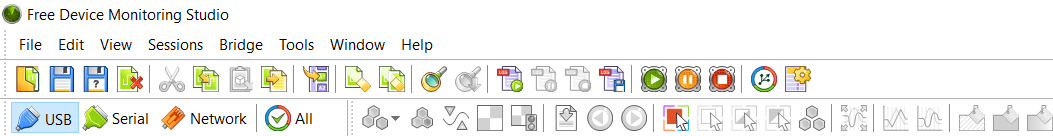
\includegraphics[width=\textwidth]{img/uvod_hhd_interface}
	\caption{Užívateľské rozhranie Device Monitoring Studio.}
	\label{obr:uvod:hhd_interface}
\end{figure}


\section{Požadované funkcie}

Ako prvé by sme si mali zadefinovať platformu na ktorú budeme cieliť s našou aplikáciou:
\begin{enumerate}[label=\textbf{P\arabic*}]
	\item \label{uvod:poz:platforma} Cieľová platforma našej aplikácie by mala byť Windows. 
\end{enumerate}

Keďže má naša aplikácia mať výukový charakter, tak sa pozrieme na typický výukový scénár jej používania. Učiteľ si dopredu do súboru zachytí komunikáciu s určitým zariadením na ktorej overí, že je didakticky dobrá a ilustruje to čo má. Následne daný súbor posunie študentom aby si mohli zobraziť analýzu konkrétnych paketov. Užitočná je ale aj analýza priamej interakcie užívateľa s jeho konkrétnym zariadením, preto by sme zároveň chceli podporovať aby si študenti mohli pripojiť vlastné zariadenie a skúmať s ním komunikáciu v reálnom čase. Z toho nám vyplývajú naledujúce požiadavky:
\begin{enumerate}[label=\textbf{P\arabic*},resume]
	\item \label{uvod:poz:analyza} Mala by byť schopná analyzovať USB pakety zachytené do~súboru v~rozumnom formáte pomocou predom definovaného snifferu.
	\item \label{uvod:poz:analyza_real_time} Mala by byť schopná analýzy paketov v reálnom čase. To znamená, že bude podporovať čítanie súboru súvisle s tým ako do neho bude zapisovať iný software (za predpokladu, že to daný software povoľuje).
\end{enumerate}

Ako sme mohli vidieť aj na predchádzajúcich príkladoch, hexdump je jednou zo základných funkcií na analýzu paketov. Zároveň sa nám ale nepáčilo, že väčšina hexdumpov je neprehľadná a ťažko sa v nich orientuje. Preto si zadefinujeme nasledujúce požiadavky:
\begin{enumerate}[label=\textbf{P\arabic*},resume]
	\item \label{uvod:poz:hexdump} Mala by pomocou hexdumpu vedieť zobraziť dáta, ktoré daný sniffer zachytí a~uloží.
	\item \label{uvod:poz:data_highlight} Mala by mať prehľadnejší hexdump a užívateľovi uľahčiť orientáciu v~ňom. Jednotlivé znaky by mali byť farebne označené na~základe ich významu (hlavička paketu, rôzne typy descriptorov a pod.).
\end{enumerate}

K sémantickej analýze sa nám môže hodiť vedieť zobraziť dáta a ich význam pomocou stromovej štruktúry. Pretože sa s našou aplikáciou budeme snažiť vysvetliť základy komunikácie na USB zbernici, mali by sme podporovať sémantickú analýzu všetkých základných USB descriptorov a takisto inputu určitej podmnožiny HID zariadení. Ako posledné by sa nám zišlo vedieť pomocou stromovej štruktúry vyobraziť hlavičku jednotlivých paketov. Z toho celého dostávame nasledovné:
\begin{enumerate}[label=\textbf{P\arabic*},resume]
	\item \label{uvod:poz:descriptory} Mala by podporovať sémantickú analýzu (vyobrazenie pomocou stromovej štruktúry) pre~všetky základné USB descriptory spomenuté v~USB 2.0 špecifikácii\cite{usbdoc} v kapitole 9.6~(ako napríklad \textit{Device descriptor}, \textit{Interface descriptor}, \textit{Endpoint descriptor}, atď.).
	\item \label{uvod:poz:hid_analyza} Mala by byť schopná pomocou stromovej štruktúry zobraziť sémantický význam dát posielaných danou podmnožinou HID zariadení, do~ktorej patrí myš, klávesnica a~joystick.
	\item \label{uvod:poz:paket_hlavicka} Mala by byť schopná pomocou stromovej štruktúry zobraziť sémantický význam jednotlivých hlavičiek paketov.
\end{enumerate}

Vyššie v texte sme označili funkciu Wiresharku vyobraziť sémantický význam dát na bitovej úrovni (obrázok~\ref{obr:uvod:byte_detail_foto}) za zaujímavú. Preto by sme ju chceli implementovať aj v našej aplikácii, z čoho vyplýva:
\begin{enumerate}[label=\textbf{P\arabic*},resume]
\item \label{uvod:poz:show_bits} V~miestach kde to dáva zmysel, by aplikácia mala byť schopná zobrazovať význam dát až na~úrovni jednotlivých bitov.
\end{enumerate}

Nechceme užívateľov hneď zaplaviť všetkými detailnými informáciami o paketoch. Preto by sme mali vedieť zobraziť zopár obecných vecí ku každému paketu a vyobraziť tak pohyb na zbernici, a až v prípade interakcie užívateľa s aplikáciou zobraziť podrobný popis jednotlivých paketov. Zároveň sa nám páčila funkcia Device Monitoring Studia, kde boli jednotlivé pakety farebne rozlišiteľné, čo zvyšovalo celkový prehľad pohybu paketov na zbernici. Z toho dostávame nasledujúce požiadavky:
\begin{enumerate}[label=\textbf{P\arabic*},resume]
	\item \label{uvod:poz:zobrazenie_paketov} Mala by na prvý pohľad jasne zobraziť základné informácie o~každom analyzovanom pakete (ako napr. dĺžka paketu, typ prenosu a pod.) a~pri~bližšom skúmaní jednotlivých paketov detailnejšie zobraziť celú jeho hlavičku. Tieto základné informácie by mali byť farebne rozlišiteľné na základe smeru paketu po zbernici.
	\item \label{uvod:poz:paket_detail} Detailnejšie informácie o~pakete budú zobrazované na~základe interakcie užívateľa s~aplikáciou.
\end{enumerate}

Aby sme boli schopní sémantickej analýzy dát myši, klávesnice alebo joysticku podľa osobného výberu užívateľa, musíme si získať informácie o ich inpute z \textit{HID Report Descriptoru}, takže naša ďalšia požiadavka je:
\begin{enumerate}[label=\textbf{P\arabic*},resume]
	\item \label{uvod:poz:report_desk_parser} Mala by byť schopná rozparsovať \textit{HID Report Descriptor} takým štýlom, aby bolo neskôr možné sématnicky reprezentovať input nami zvolených HID zariadení -- myš, klávesnica a joystick.
\end{enumerate}

\section{Ciele práce}

Celkové ciele tejto práce sú následovné :

\begin{enumerate}[label=\textbf{C\arabic*}]
	\item \label{uvod:ciel:aplikacia} Naprogramovať funkčný analyzátor, ktorý spĺňa všetky požadované funkcie~\ref{uvod:poz:platforma}\=/\ref{uvod:poz:report_desk_parser}
	\item \label{uvod:ciel:rozsiritelnost} Návrh programu musí byť dostatočne obecný aby splňoval nasledujúce:
	\begin{itemize}
		\item \label{uvod:ciel:roz_USB} Jednoduché rozšírenie o~analýzu ďalších typov USB prenosov.
		\item \label{uvod:ciel:roz_HID} Jednoduché pridanie sémantickej analýzy pre~ďalšie HID zariadenia.
	\end{itemize}
\end{enumerate}
\chapter{USB a Windows}
vysvetlenie zakladnych pojmov spojenych USB: historia, usb port/conector, plug and play(https://docs.microsoft.com/en-us/windows-hardware/drivers/kernel/introduction-to-plug-and-play), low/full/high speed zariadenia
\section{USB zbernica}
Plug and Play device tree(sposob akym si windows udrziava strom zariadeni na zbernici)(https://docs.microsoft.com/sk-sk/windows-hardware/drivers/gettingstarted/device-nodes-and-device-stacks)
\section{Device object a device stack}
PDO,FDO, Device object(https://docs.microsoft.com/en-us/windows-hardware/drivers/kernel/introduction-to-device-objects)
https://docs.microsoft.com/en-us/windows-hardware/drivers/kernel/creating-a-device-object
\subsection{Drivery}
Opisat ako teda bezne analyzatory/sniffery funguju
windows driver model(WDM) : https://docs.microsoft.com/en-us/windows-hardware/drivers/kernel/types-of-wdm-drivers
bus driver(https://docs.microsoft.com/en-us/windows-hardware/drivers/kernel/bus-drivers), function driver(https://docs.microsoft.com/en-us/windows-hardware/drivers/kernel/function-drivers) a filter driver(https://docs.microsoft.com/en-us/windows-hardware/drivers/kernel/filter-drivers)
\section{Komunikacia s USB zariadenim}
sposob komunikacie operacneho systemu so zariadenim pripojenym na USB zbernicu : IRP(https://docs.microsoft.com/en-us/windows-hardware/drivers/gettingstarted/i-o-request-packets) , URB (https://docs.microsoft.com/en-us/windows-hardware/drivers/usbcon/communicating-with-a-usb-device) a pod.
https://docs.microsoft.com/en-us/windows-hardware/drivers/kernel/handling-irps
\section{USB descriptory}
opis zakladnych USB descriporov, hlavne tych ktore neskor aj vyuzivam v program(Device, Interface, Endpoint, Configuration, String, Setup) : https://docs.microsoft.com/en-us/windows-hardware/drivers/usbcon/usb-descriptors
https://docs.microsoft.com/en-us/windows-hardware/drivers/usbcon/usb-control-transfer
\subsection{Rozlozenie USB zariadenia z hladiska descriptorov}
https://docs.microsoft.com/en-us/windows-hardware/drivers/usbcon/usb-device-layout
\section{HID zariadenia}
hid zariadenie obecne, priklady
https://docs.microsoft.com/en-us/windows-hardware/drivers/hid/
\subsection{Reporty}
Input/Output/Feature reporty.
\subsection{Report Descriptor}
Opis report descriptoru, k comu sluzi, pripadne ako z neho vycitat zaujimave data (neskor vyuzite v programe pri parsovani HID Report Descriptoru na naslednu semanticku analyzu dat ktore posiela zariadenie)






\chapter{Analýza}
\section{Získanie USB packetov}
Na získavanie USB paketov nám bude obecne slúžiť paket sniffer. Väčšina paket analyzátorov má implementované vlastné sniffery a preto sme sa o to pokúsili tiež. Narazili sme ale na niekoľko zásadných problémov, ktoré sa úzko viažu s platformou na ktorú cielime s našou aplikáciou~--~Windows.

Microsoft dokumentácia podrobnejšie opisuje komunikáciu medzi HID zaridením a kernel/user-mode aplikáciou~\cite{hid_opening_collections}. Keďže naša aplikácia beží v user-mode, prejdeme si tento spôsob:
\begin{enumerate}
\item Aplikácia nájde a identifikuje HID zariadenie.
\item Aplikácia pomocou metódy \textit{CreateFile} otvorí spojenie s HID zariadením.
\item Aplikácia pomocou \textit{HID API}~\cite{hid_api} metód \textit{HidD\_Xxx} získa \textit{Preparsed Data} a informácie ohľadom HID zariadenia.
\item \textbf{Aplikácia použije metódu \textit{ReadFile} resp. \textit{WriteFile} na získanie inputu zariadenia resp. poslanie reportu zariadeniu.}
\item Aplikácia pomocou \textit{HID API}~\cite{hid_api} metód \textit{HidP\_Xxx} interpretuje HID reporty.
\end{enumerate}

\subsection{Windows exclusive mód}
Windows má definovaný tzv. \textit{Access Mode}, ktorý určuje restrikciu prístupu \textit{HID Clienta} k HID zariadeniu. 
Ten môže byť buď \textit{Shared} alebo \textit{Exclusive}. \textit{Exclusive Mode} zabraňuje ostatným \textit{HID Clientom} v zachytávaní alebo získavaní inputu HID zariadenia, pokiaľ nie sú hlavným príjemcom daného inputu. Preto z bezpečnostných dôvodov otvára \textit{RIM (Raw Input Manager)} niektoré zariadenia v \textit{Exclusive Mode}.

Ak je zariadenie otvorené v \textit{Exclusive Mode}, aplikácia má stále prístup k niektorým jeho údajom pomocou  \textit{HID API}~\cite{hid_api} metód  \textit{HidD\_\textbf{Get}Xxx}. Tieto metódy nám obecne umožnia získať niektoré descriptory zariadenia, tak ako aj jeho \textit{Preparsed Data}. Nie je nám ale umožnené volať metódu \textit{ReadFile}, takže nemáme akým spôsobom zachytávať komunikáciu HID zariadenia s clientom.

Tabuľka zariadení~\cite{hid_access} (obrázok~\ref{obr:kap3:access_mode}), ktoré \textit{RIM} otvára v \textit{Exclusive Mode} obsahuje aj tie, ktoré sme si v úvode zvolili ako podmnožinu HID zariadení na analýzu -- myš a klávesnica.

\begin{figure}[!htb]
	\centering
	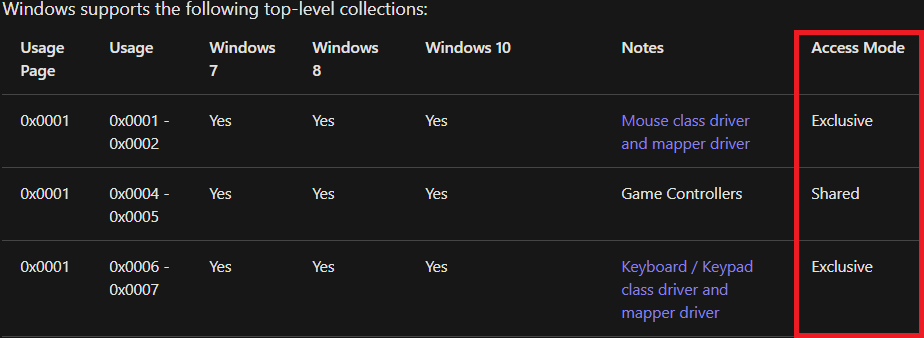
\includegraphics[width=\textwidth]{img/kap3_access_mode}
	\caption{Tabuľka zariadenía ich \textit{Access Mode}. Zariadenia postupne po riadkoch -- myš, joystick a klávesnica}
	\label{obr:kap3:access_mode}
\end{figure}

\newpage

\subsection{Známe knižnice}
opisat zakladne kniznice na sledovanie USB zbernice a preco som ich nemohol pouzit : libUSB, hidAPI

\subsection{Driver}
TU povedat riesenie - pouzitie driveru na komunikaciu so zariadenim. Existujuce windows drivery -- moufiltr, Kbdfiltr - nefunguju pre USB

TU spomenut posledne mozne riesenie - napisanie vlastneho filter driveru. 

\subsection{Third-party aplikácie}
opisat odkial nakoniec ziskavam packety - USBPcap a Wireshark









\section{Spracovávanie pcap súborov}
moznosti ako citat pcap subory : bud pouzit uz existujucu kniznicu : na linuxe Libpcap, windows NPcap(deprecated WinPcap), alebo citat subory manualne : std::istream alebo QFile
\section{Sémantická reprezentácia dát}
ako si z dat vytiahnut udaje ktore su potom pouzite na semanticku analyzu implementovanych HID zariadeni : HID Report parser, InputValues a EndpointDevice struct.
Nasledne sparovanie - ako vybrat spravny report pre konkretny input
\section{Voľba frameworku}
obecne co by som od toho GUI priblizne chcel, potom opisat preco som si vybral prave Qt a v nasledujucich kapitolach opisat rozhodnutia uz v Qt
dovod preco som si zvolil qt namiesto inych c++ GUI frameworkov(napriklad sfml)
\section{Zobrazenie základných informácií}
ako zobrazovat zakladne info o packete : pouzit QListWidget alebo QTableWidget (pripadne nieco ine ako nejaky abstract viewmodel), narok na zakladne funkcionality : lahka rozsiritenlnost o dalsie ''stlpceky'' , moznost jednoduchej interakcie(doubleClick na polozku). Mat vsetky info na jednom okne / mat pop-up okna.
\section{Zobrazenie sémantického významu dát}
ako vyzobrazit semanticky vyznam roznych dat - descriptory, usb header, vyznam input dat roznych HID zariadeni
\section{Hexdump}
ako v qt urobit hexdump - do coho zobrazovat data(vytvorit si vlastny viewer dedeny od QAbstractScrollArea, pripadne niecoho ineho) vs najst nieco co uz v qt je a upravit to aby to sedelo poziadavkam. Vziat do uvahy bezne funkcie hexdumpu : selection mody(oznacit naraz hexa a im odpovedajuce printable), logicke oddelenie dat(napriklad farbami)









\chapter{Vývojová dokumentácia}
\label{chap:vyvoj_dok}
\section{Architekrúra aplikácie}
\section{Jadro aplikácie}
\subsection{USB\_Packet\_Analyzer}
riadi celkovy beh programu, reaguje na input od uzivatela
\subsection{Item Manager}
spracovanie samostatneho packetu a ulozenie dat o nom
\subsection{DataViewer}
trieda ktora ma na starosti vyskakovacie okno po dvojkliku a item a nasledne reaguje na input od uzivatela v okne
\subsection{TreeItem}
reprezentuje jednotlive nody v stromovej strukture ktora sa potom vyuziva na zobrazenie dat v QTreeView
\section{Modely}
\subsection{AdditionaldataModel}
model na spravovanie zvysnych dat(data ktore nie su sucastou hlavicky packetu)
\subsection{ColorMapModel}
vyobrazenie pomocnej mapy na lepsie sa zorientovanie v zvyraznemom hexdumpe
\subsection{DataViewerModel}
model na hexdump - prenasa hex/printable a zaroven o co vlastne ide(konkretny descriptor, interrupt data, ...)
\subsection{TreeItemBaseModel}
model na QTreeView ktorz vyuziva TreeItem
\subsection{USBPcapHeaderModel}
model na QTreeView ale specialne pre USBPcap hlavicku packetu
\section{Interpretery}
\subsection{BaseInterpreter}
abstractna trieda od ktorej dedia vsetkz interpretery
\subsection{Interpreter factory}
facory trieda na pridelenie konkretneho interpreteru za runtimu kvoli jednoduchosti na lepsie rozsirenie programu do buducnosti
\subsection{Interpretery descriptorov}
Config,Device,Setup,String,...
\subsection{Interrupt transfer interpretery}
obecne interrupt transfer interpreter - sluzi skor ako factory na rozne doteraz implementovane HID zariadenia
\subsubsection{Joystick interpreter}
\subsubsection{Mouse interpreter}
\subsubsection{Keyboard interpreter}
\section{Delegáti}
\subsubsection{DataViewerDelegate}
Qt delegat - stara sa o highlight hexdumpu
\section{HID}
\subsection{HIDDevices}
staticka trieda, drzi vsetky rozpoznane HID zariadenia a obsahuje funkcie specificke nich - parsovanie HID Report descriptoru
\section{Práca so súbormi}
\subsection{FileReader}
praca zo suborom a predavanie precitanych dat, offline/online capture, QFile vs std::istream
\section{Globálne dáta}
\subsection{ConstDataHolder}
staticka trieda na drzanie si konstant ktore su potrebne napriec celym programom. Mapovanie z enumu do jeho stringovej reprezentacie
\subsection{PacketExternStructs}
obsahuje definiciu vsetkych dolezitych USBPcap structov, pcap structov, enumov a vsetkych structov ktore pouzivam v aplikacii












\chapter{Možnosti rozšírenia}
Rozobrať čo všetko sa dá urobiť s tými dátami, ktoré už mám uložené v pamati, ale momentálne sa s nimi nič nedeje
\section{Ukladanie výstupu do súboru}
výstup analýzy do súboru(textového)
\section{Iná vizuálna reprezentácia dát}
Momentálne vyzobrazujem dáta prevažne v QTreeView alebo QTableView, ale vdaka tomu ako ich mám uložené + to že nad nimi operuje nejaký model ktorý vie vrátiť dáta na základe indexu, by nemuselo byť taká zložité pridať inú vizualizáciu dát(napríklad obrázkovú ako tu : https://www.usbmadesimple.co.uk/ums\_5.htm)
\section{Pridávanie nových interpreterov pre descriptory}
pridanie nových druhov descriptorov - pridať nový interpreter do factory
\section{Pridanie intepreteru na interrupt tranfser}
pridanie analyzy interrupt transferu aj pre ine ako hid zariadenia
\subsection{Pridanie nových HID zariední}
nove HID zariadenie - pridanie do interrupt ''factory''
\section{Pridanie analýzy pre isochronous a bulk transfer}
semanticka analyza aj inych ako interrupt alebo control transferov - momentalne su rozpoznavane len v hexdumpe
\section{?Možnosť rozšírenia na iné platformy?}
uprava aplikacie aby bola prenositelna aj na ine platformy, co vsetko by tam bolo treba upravit(pravdepodobne nie vela, kedze qt je prenosne, a prakticky jedine co pouzivam spojene s windowsom su jeho structy na rozne descriptory)

\chapter{Užívateľská dokumentácia}
\section{Inštalácia}
nastavenie celkovej aplikácie, ale aj nainstalovanie USBPcap + wireshark a ich kombinácia pre live capture
\section{Orientácia v GUI aplikácie}
popis k jednotlivým tlačidlám gui
\section{Používanie aplikácie}
ako spustit live/offline capture, a celkovo ako pracovať s aplikáciou(popis funkcií - doubleClick na item => zobrazi sa pop-up okno s bližšou analýzou)




\chapter{Záver}
\section{Zhrnutie}
celkove zhrnutie prace, ?praca s Qt?
\section{Budúce plány}




%%% Seznam použité literatury
%%% Seznam použité literatury (bibliografie)
%%%
%%% Pro vytváření bibliografie používáme bibTeX. Ten zpracovává
%%% citace v textu (např. makro \cite{...}) a vyhledává k nim literaturu
%%% v souboru literatura.bib.
%%%
%%% Příkaz \bibliographystyle určuje, jakým stylem budou citovány odkazy
%%% v textu. V závorce je název zvoleného souboru .bst. Styly plainnat
%%% a unsrt jsou standardní součástí latexových distribucí. Styl czplainnat
%%% je dodáván s touto šablonou a bibTeX ho hledá v aktuálním adresáři.

% \bibliographystyle{czplainnat}    %% Autor (rok) s českými spojkami
% \bibliographystyle{plainnat}    %% Autor (rok) s anglickými spojkami
\bibliographystyle{unsrt}       %% [číslo]

\renewcommand{\bibname}{Zoznam použitej literatúry}

%%% Vytvoření seznamu literatury. Pozor, pokud jste necitovali ani jednu
%%% položku, seznam se automaticky vynechá.

\bibliography{outro/literatura}

%%% Kdybyste chtěli bibliografii vytvářet ručně (bez bibTeXu), lze to udělat
%%% následovně. V takovém případě se řiďte normou ISO 690 a zvyklostmi v oboru.

% \begin{thebibliography}{99}
%
% \bibitem{lamport94}
%   {\sc Lamport,} Leslie.
%   \emph{\LaTeX: A Document Preparation System}.
%   2. vydání.
%   Massachusetts: Addison Wesley, 1994.
%   ISBN 0-201-52983-1.
%
% \end{thebibliography}


%%% Obrázky v bakalářské práci
%%% (pokud jich je malé množství, obvykle není třeba seznam uvádět)
\listoffigures

%%% Tabulky v bakalářské práci (opět nemusí být nutné uvádět)
%%% U matematických prací může být lepší přemístit seznam tabulek na začátek práce.
\listoftables

%%% Použité zkratky v bakalářské práci (opět nemusí být nutné uvádět)
%%% U matematických prací může být lepší přemístit seznam zkratek na začátek práce.
\chapwithtoc{Seznam použitých zkratek}

%%% Přílohy k bakalářské práci, existují-li. Každá příloha musí být alespoň jednou
%%% odkazována z vlastního textu práce. Přílohy se číslují.
%%%
%%% Do tištěné verze se spíše hodí přílohy, které lze číst a prohlížet (dodatečné
%%% tabulky a grafy, různé textové doplňky, ukázky výstupů z počítačových programů,
%%% apod.). Do elektronické verze se hodí přílohy, které budou spíše používány
%%% v elektronické podobě než čteny (zdrojové kódy programů, datové soubory,
%%% interaktivní grafy apod.). Elektronické přílohy se nahrávají do SISu a lze
%%% je také do práce vložit na CD/DVD. Povolené formáty souborů specifikuje
%%% opatření rektora č. 72/2017.
\appendix
%%% Přílohy k bakalářské práci, existují-li. Každá příloha musí být alespoň jednou
%%% odkazována z vlastního textu práce. Přílohy se číslují.
%%%
%%% Do tištěné verze se spíše hodí přílohy, které lze číst a prohlížet (dodatečné
%%% tabulky a grafy, různé textové doplňky, ukázky výstupů z počítačových programů,
%%% apod.). Do elektronické verze se hodí přílohy, které budou spíše používány
%%% v elektronické podobě než čteny (zdrojové kódy programů, datové soubory,
%%% interaktivní grafy apod.). Elektronické přílohy se nahrávají do SISu a lze
%%% je také do práce vložit na CD/DVD. Povolené formáty souborů specifikuje
%%% opatření rektora č. 72/2017.

\chapwithtoc{Prílohy}

\section{První příloha}

\openright
\end{document}
